\bibliographystyle{plunsrt}
\renewcommand{\autorzy}{M.~Nowak, G.~Maj}
\chapter[Audyt w systemach informatycznych][Audyt w systemach informatycznych]{Audyt w systemach informatycznych}

  Jednym z podstawowych problemów profesjonalnego zarz¹dzania firm¹ w~bran¿y informatycznej jest zarz¹dzanie jakoœci¹. Jakoœæ mo¿na definiowaæ i~mierzyæ na wielu poziomach. Bardzo du¿o uwagi poœwiêcane jest jakoœci produktów, choæ równie wa¿nym elementem jest ocena jakoœci pracy pracowników oraz ich efektywnoœci. Audyt w systemach informatycznych powinien zawieraæ tak¿e elementy oceny jakoœci pracy i s³u¿yæ usprawnieniu dzia³ania organizacji.

W rozwa¿aniach na temat oceny jakoœci pracy i wydajnoœci pracowników skupiono siê na firmach informatycznych, których przedmiotem dzia³alnoœci jest wytwarzanie oprogramowania. Kluczowym pracownikiem bior¹cym udzia³ w~tworzeniu koñcowego produktu, czyli programu jest programista. Ocena pracy programisty jest zadaniem z³o¿onym i wymaga znajomoœci wielu aspektów procesu wytwarzania oprogramowania. W dzisiejszych czasach zarz¹dzanie jakoœci¹ oprogramowania jest prawdziwym wyzwaniem dla du¿ych firm o zasiêgu globalnym zatrudniaj¹cych tysi¹ce programistów z ca³ego œwiata.

Podstawowym pytaniem, które postawiono w tym rozdziale jest: jak efektywnie mierzyæ jakoœæ i efektywnoœæ pracy programisty? W niniejszym artykule autorzy postaraj¹ siê przybli¿yæ problem, przedstawiæ dostêpne na rynku rozwi¹zania oraz opisaæ prosty system kontroli efektywnoœci pracy.


\section{Dostêpne systemy pomiaru pracy}
\label{sec:dostepneSystemy}

Na rynku istniej¹ ró¿ne systemy s³u¿¹ce do pomiaru i wspomagania pracy programisty. Skupiaj¹ siê one
g³ównie na ³¹czeniu kodu i kontroli pracy wielu programistów, pracuj¹cych nad jednym projektem. Poni¿ej przedstawione zosta³y najpopularniejsze systemy, w tym rozbudowane i szeroko wykorzystywane systemy otwartoŸród³owe.

\subsection{Systemy kontroli wersji}

Systemy kontroli wersji stworzone s¹ do pomocy przy rozwoju oprogramowania, ich g³ównym zadaniem jest ³¹czenie pracy wielu pracowników jednego projektu, jednak poprzez tworzenie historii zmian w projekcie daje mo¿liwoœæ kontroli i oceny pracy pracowników.
Daj¹ one mo¿liwoœæ œledzenia postêpu prac poczynionych przez poszczególnych pracowników. Podstawowe informacje, które mo¿na uzyskaæ to:
\begin{itemize}
	\item jaki u¿ytkownik i kiedy wprowadza³ zmiany,
	\item mo¿liwoœæ sprawdzenia jakie zmiany zosta³y wprowadzone w danym commicie:
	\begin{itemize}
		\item dok³adne ró¿nice miêdzy zmienionymi plikami,
		\item skrócone statystyki(iloœæ zmian bez poszczególnych ró¿nic),
		\item sumy kontrolne poszczególnych zmian,
		\item wyœwietlanie tylko informacji przez nas okreœlonych,
	\end{itemize}
	
	\item mo¿liwoœæ dostosowania informacji przez nas œledzonej: 
	\begin{itemize}
		\item kontrola jednego pracownika,
		\item kontrola danego okresu zmian,
		\item kontrola historii tworzenia i ³¹czenia ga³êzi.
	\end{itemize}

\end{itemize}

Przyk³adami systemów kontroli wersji s¹ najbardziej popularne darmowe systemy takie jak: Git
\cite{website:git}, Svn \cite{website:svn} czy  Mercurial \cite{website:mercurial}.



	\subsubsection{Git}
	Git jest rozproszonym systemem kontroli wersji. Jest to wolne oprogramowanie udostêpnione na licencji
	GNU GPL2. Git powsta³ jako alternatywa dla zamkniêtego systemu BitKeeper w kwietniu 2005 roku do
	rozwijania projektu Linux.
	
	\subsubsection{Svn}
	Subversion jest wolnym systemem kontroli wersji udostêpnionym na licencji Apache. Zosta³ stworzony do
	zast¹pienia systemu CVS.
	
	\subsubsection{Mercurial}
	Marcurial podobnie jak Git jest rozproszonym systemem kontroli wersji. Zosta³ napisany w tym samym
	czasie jak Git, równie¿ w celu pomocy do rozwijania projektu Linux. Jest wykorzystywany w wielu projektach
	otwartoŸród³owych.

\subsection{Systemy zarz¹dzania projektem}

Systemy zarz¹dzania projektem s¹ platformami wspomagaj¹cymi podzia³ prac i weryfikacjê postêpów prac.
Z tego tytu³u daj¹ pewien obraz pracy w³o¿onej przez ka¿dego wspó³pracownika. Poni¿ej zosta³y przedstawione najpopularniejsze systemy zarz¹dzania:

\begin{itemize}
	\item \textbf{Redmine}
	
	Redmine \cite{website:redmine} jet wolnym, otwartoŸród³owym internetowym narzêdziem do zarz¹dzania projektem i szukania
	b³êdów. Udostêpnia kalendarz i wykres Ganta wraz ze wsparciem wizualnym by ³atwiej kontrolowaæ
	koñcz¹ce siê etapy projektu. Wspiera ró¿ne systemy kontroli wersji i umo¿liwia kontrole nad podzia³em
	zadañ w grupie. Narzêdzie Redmine jest oparte o framework Ruby on Rails, co zapewnia mu przenoœnoœæ.

	
	\item \textbf{Jira}
	
	JIRA \cite{website:jira} jest zamkniêtym oprogramowaniem stworzonym przez firmê Atlassian, które ma na celu wspomaganie w
	zarz¹dzaniu projektem i œledzeniu b³êdów. Jest wykorzystywana w wielu projektach m.in. Fedora
	Commons, Skype czy JBoss. Jest narzêdziem wieloplatformowym dziêki oparciu go o jêzyk Java. Firma
	Atlassian  udostêpnia program JIRA nieodp³atnie do u¿ytku non-profit.


	\item \textbf{GitHub}
	
	GitHub \cite{website:github} jest serwisem hostingowym dla projektów wykorzystuj¹cych system kontroli wersji Git. Udostêpnia
	darmowe otwarte repozytoria a tak¿e p³atne repozytoria zamkniête. Oprócz podstawowego zadania jakim
	jest przechowywanie plików projektu wspomaga kontrolê nad tworzeniem oprogramowania poprzez dodatkowe
	narzêdzie nieobecne w systemie Git np. bugtracker, forki repozytoriów, graficzne statystyki czy wiki z
	dokumentacj¹. Umo¿liwia ³¹czenie programistów w organizacje i przydzielanie mo¿liwoœci rozwijania 
	oprogramowania dla konkretnych u¿ytkowników.

\end{itemize}


\subsection{Systemy do statycznej analizy kodu}

Platformami najbardziej zbli¿onymi do zmian w samym kodzie projektu, a~nie tylko du¿ymi zmianami w
strukturze ca³ego projektu, b¹dŸ gotowymi dzia³aj¹cymi zmianami obserwowanymi poprzez zmianê plików w 
repozytorium, s¹ systemy do statycznej analizy kodu. Ich cech¹ jest praca równolegle do tworzonego kodu, a 
nie obserwacja zmian etapami. Obecnie s¹ powszechnie dostêpne platformy obs³uguj¹ce wszystkie popularne 
jêzyki programowania. Przyk³adami takich systemów s¹:

\begin{itemize}
	\item \textbf{Klocwork}
	
	Klocwork \cite{website:klocwork} jest zamkniêtym programem przeznaczonym do statycznej analizy kodu pozwalaj¹cym na detekcjê
	b³êdów strukturalnych kodu i b³êdów przebiegu programu. Umo¿liwia pracê z najpopularniejszymi jêzykami
	C, C++, Java czy C\#.
		 
	\item \textbf{Pylint}
	
	Pylint \cite{website:pylint} jest otwrtoŸród³owym oprogramowaniem do znajdywania b³êdów w~kodzie i~sprawdzania jego jakoœci.
	Pylint jest podobny do innego oprogramowania Pychecker ale jest bardziej rozbudowany. Wspiera miêdzy
	innymi sprawdzanie d³ugoœci linii, sprawdzanie zgodnoœci nazw zmiennych ze standardem kodowania czy 
	tworzenie diagramów UML ze stworzonego kodu.
	
	\item \textbf{CodeSonar}
	
	CodeSonar \cite{website:codesonar} jest zamkniêtym oprogramowaniem analizuj¹cym kod pod wzglêdem bezpieczeñstwa i poprawnoœci.
	Wspiera oprogramowanie napisane w C, C++ i Java. Jest wykorzystywany w wielu ga³êziach gospodarki
	m.in.~w~NASA czy w firmie Toyota. Oprócz analizy kody umo¿liwia wizualizacjê architektury programu i
	zbiera dane do metryk oceny jakoœci kodu.
	
\end{itemize}


\section[Sposoby pomiaru jakoœci pracy programisty][Sposoby pomiaru jakoœci pracy programisty]
{Sposoby pomiaru jakoœci pracy programisty}
\label{sec:sposobyPomiaruJakosci}
Na ocenê pracownika programisty mo¿na patrzeæ z ró¿nych perspektyw. Z~jednej strony, efektem jego
pracy jest kod Ÿród³owy, wiêc podstawowym sk³adnikiem oceny powinna byæ jego jakoœæ. Z drugiej
strony jednak, w ka¿dym projekcie obecne s¹ pewne ograniczenia czasowe, wiêc szybkoœæ pracy
pracownika jest równie¿ wa¿nym aspektem oceny. W ogólnoœci mo¿na powiedzieæ, ¿e jakoœæ pracy
programisty mo¿na sprowadziæ do dwóch sk³adników:
\begin{itemize}
	\item oceny jakoœci kodu,
	\item oceny organizacji pracy.
\end{itemize}

Normy dotycz¹ce zarz¹dzania jakoœci¹ (np. ISO 9000:2008, ISO 15504-4:2005) definiuj¹ tzw. kluczowe 
wskaŸniki efektywnoœci (ang. KPI - key performance indicator). Wa¿n¹ cech¹ tych wskaŸników jest
to, ¿e opisuj¹ one mierzalne procesy w postaci liczbowej. Daje to mened¿erowi obiektywny obraz
efektywnoœci danego procesu w przedsiêbiorstwie i pozwala na cykliczn¹ kontrolê jakoœci. Poni¿ej
przedstawiono kilka przyk³adowych wskaŸników, które spe³niaj¹ warunek mierzalnoœci, wiêc kwalifikuj¹
siê do grupy KPI. 

\subsection[Ocena jakoœci wygenerowanego kodu][Ocena jakoœci wygenerowanego kodu]{Ocena jakoœci 
wygenerowanego kodu}
\label{subsec:ocenaJakosciKodu}
Jakoœæ kodu jest bardzo szerokim zagadnieniem, które po wielu dekadach intensywnego rozwoju bran¿y
IT nie zosta³o jeszcze dostatecznie zbadane. Wynika to st¹d, ¿e na przestrzeni lat zmienia³y siê
trendy w tworzeniu oprogramowania -- programiœci stosowali ró¿ne paradygmaty programowania (w 
kolejnoœci chronologicznej: programowanie obiektowe, programowanie strukturalne, programowanie 
funkcjonalne). Dziœ dominuj¹cym paradygmatem jest programowanie obiektowe, lecz wydaje siê, ¿e 
prawdziwa jest teza, ¿e ka¿da z wymienionych filozofii tworzenia oprogramowania jest u¿yteczna dla
pewnych zastosowañ.

St¹d obiektywny pomiar jakoœciowy kody jest trudny. Niektóre elementy jêzyka mog¹ byæ uznawane za
wartoœciowe w jednym podejœciu, a drugim absolutnie niedopuszczalne. Istniej¹ jednak pewne
fundamentalne cechy kodu, które s¹ po¿¹dane zawsze, np. zwiêz³oœæ kodu.

Wartoœci s³u¿¹ce do pomiaru pewnej w³asnoœci oprogramowania lub jego specyfikacji nazywane s¹
metrykami oprogramowania. Aby metryka by³a u¿yteczna powinna byæ:
\begin{itemize}
	\item prosta i mo¿liwa do obliczenia przez komputer,
	\item przekonuj¹ca,
	\item konsekwentna i obiektywna,
	\item spójna pod wzglêdem u¿ytych jednostek,
	\item niezale¿na od jêzyka oprogramowania,
	\item daj¹ca przydatne informacje \cite{website:metric}.
\end{itemize}

Metryki mo¿na podzieliæ na statyczne i dynamiczne. Metryki statyczne ³¹cz¹ siê œciœle z analiz¹ 
statyczn¹ kodu, dziedzin¹ in¿ynierii oprogramowania zajmuj¹c¹ siê badaniem struktury kodu 
Ÿród³owego. Metryki te najbardziej przydatne s¹ dla samych programistów i innych osób bezpoœrednio
zaanga¿owanych w proces powstawania oprogramowania. Pozwalaj¹ na bie¿¹ce œledzenie jakoœci kodu i
zwrócenie uwagi na miejsca, które wymagaj¹ uproszczenia b¹dŸ szczególnie uwa¿nego testowania.
Niemniej jednak, programista, który dostarcza kod o dobrych statycznych metrykach mo¿e byæ uznawany
za dobrego pracownika.

Metryki dynamiczne to wskaŸniki abstrahuj¹ce od kodu Ÿród³owego. Badaj¹ one zachowanie programu po
jego uruchomieniu. S¹ one mocno zwi¹zane z wymaganiami klienta, st¹d dla samego przedsiêbiorcy,
s¹ to liczby przydatne bardziej do analizy jakoœci produktu ni¿ pracy jego pracowników.  

\subsubsection[Linie kodu (LOC)][Linie kodu (LOC)]{Linie kodu (LOC)}
\label{subsubsec:linieKodu}
Najprostsz¹ metryk¹ rozmiaru oprogramowania jest liczba linii kodu Ÿród³owego. Mimo jej prostoty,
wymaga ona pewnego rozró¿nienia, bowiem programy pisane w jêzykach wysokiego poziomu maj¹ znacz¹co
mniej linii kody ni¿ programy pisane np. w assemblerze. Do tej metryki z regu³y nie s¹ wliczane
równie¿ linie zawieraj¹ce tylko komentarze.

Wa¿nym aspektem jest tutaj równie¿ styl pisania kodu. Poni¿sze dwa przyk³ady obrazuj¹ dwa ró¿ne
style programowania w jêzyku C++ obrazuj¹ce ten niuans:

\begin{lstlisting}
// przyklad 1
void bubblesort(std::vector<int>& A)
{
	int temp = 0;

	for (int i = 0; i < A.length()-1; i++)
	{
		for (int j = 0; j < A.length()- 1 - i; j++)
		{
			if (A[j] > A[j+1])
			{
				temp = A[j+1];
				A[j+1] = A[j];
				A[j] = temp;
			}
		}
	}
}
\end{lstlisting}

\begin{lstlisting}
// przyklad 2
void bubblesort(std::vector<int>& A) {
	for (int i = 0; i < A.length()-1; i++)
		for (int j = 0; j < A.length()- 1 - i; j++)
			if (A[j] > A[j+1])
				std::swap(A[j], A[j+1]);
}
\end{lstlisting}

Oba przyk³ady s¹ identyczn¹ implementacj¹ popularnego algorytmu sortowania b¹belkowego. W pierwszym
przyk³adzie stosowane s¹ przeniesienia do nastêpnej linii przy otwieraniu nowych bloków kodu (klamr
\{\}). Oprócz tego, ka¿de wyra¿enie warunkowe i pêtle s¹ akcentowane nowym otwarciem i zamkniêciem
klamry, choæ sk³adnia jêzyka C++ tego nie wymaga. Dodatkowo, w~drugim przyk³adzie, aby bardziej
zwiêkszyæ zwiêz³oœæ (i czytelnoœæ) kodu, do operacji zamiany wartoœci dwóch elementów wektora,
zastosowano funkcjê z biblioteki standardowej, która ma dok³adnie takie samo dzia³anie jak kod
z przyk³adu pierwszego.

\subsubsection[Linie kodu na plik Ÿród³owy (LOCPF)][Linie kodu na plik Ÿród³owy (LOCPF)]
{Linie kodu na plik Ÿród³owy (LOCPF)}
\label{subsubsec:linieKoduNaPlik}

Kolejn¹ metryk¹ zwi¹zan¹ z iloœci¹ linii kodu w plikach jest miara iloœci linii kodu na plik.
Metryka ta jest szczególnie wa¿na ze wzglêdu na to, ¿e zapewnia ewaluacjê projektu programistycznego
jako ca³oœci. Wa¿ne jest, aby nie wliczaæ do tej metryki plików konfiguracyjnych ani plików
wynikowych budowania.

Do wyliczenia LOCPF mo¿na wykorzystaæ metrykê LOC:
\begin{align*}
    &\frac{1}{N}\sum_{f=1}^NLOC(file[f]) \quad f: file[f] \in source\_files
\end{align*}


\subsubsection[Brak spójnoœci metod (LCOM)][Brak spójnoœci metod (LCOM)]
{Brak spójnoœci metod (LCOM)}
Metryka ta bazuje na tezie, ¿e wszystkie metody powinny byæ spójne. St¹d nazwa LCOM (\textit{Lack of 
Cohesion of Methods}). Spójnoœæ metody oznacza ¿e ma ona jedn¹ kompetencjê i nie wchodzi w
kompetencje innych metod. Tak organizowany kod jest dobrze zrefaktoryzowany, a przez to ³atwiej
utrzymywalny, testowalny oraz czytelny.

Spójnoœæ metod (a tak¿e klas i innych obiektów jêzyka) jest cech¹, o której mówi jedna z zasad
architektury SOLID -- Single Responsibility Principle (SRP). Architektura, która przestrzega zasad
SOLID cechuje siê du¿¹ stabilnoœci¹ oprogramowania i elastycznym designem\cite{book:agile}.

Jak wskazuje sama nazwa, metryka ta opisuje brak spójnoœci, a wiêc po¿¹dane jest, aby by³a jak
najmniejsza. Jest kilka sposobów jej obliczania. Poni¿ej przedstawiono jedn¹ z bardziej przejrzystych. Definiuje siê:
\begin{itemize}
    \item $m$ -- liczba metod w klasie,
    \item $a$ -- liczba atrybutów w klasie,
    \item $mA(a)$ -- liczba metod maj¹cych dostêp do atrybutu $a$,
    \item $sum(mA)$ -- suma wartoœci $mA$ po wszystkich atrybutach.
\end{itemize}
Wówczas:
\begin{equation*}
    LCOM = 1 - \frac{sum(mA)}{m \times a}
\end{equation*}

\subsection{Ocena efektywnoœci pracy}
\label{subsec:ocenaEfektywnosci}
Problem oceny efektywnoœci pracy programisty nie jest problemem ³atwym. Dosyæ prosto mo¿na
zaproponowaæ podstawowe kryteria jednak nie zawsze oddaj¹ one faktyczny nak³ad pracy. 

\begin{itemize}
	\item czas pracy pracownika,
	\item iloœæ rozwi¹zanych zadañ,
	\item efektywnoœæ mierzona stosunkiem predyktywnoœci do wykonanych zadañ,
	\item ocena wygenerowanego kodu:
	\begin{itemize}
		\item iloϾ wygenerowanego kodu,
		\item rozk³ad kodu w plikach,
		\item przejrzystoϾ kodu,
		\item jakoœæ testów,
		\item jakoϾ dokumentacji,
		\item nazewnictwo funkcji i klas,
		\item analiza statyczna kodu,
	\end{itemize}
\end{itemize}



\section{Proponowane rozwi¹zanie}
\label{sec:czwarta}

W niniejszej pracy utworzono wtyczkê do popularnego œrodowiska programistycznego Eclipse. Wtyczka pozwala 
na analizê rozk³adu kodu w projekcie. Przegl¹da wszystkie pliki Ÿród³owe w przestrzeni pracy, tworzy
historiê zmiany plików i pozwala na przejrzyst¹ wizualizacjê zebranych danych.

	\subsection{Eclipse IDE}
	
	Eclipse \cite{website:eclipse} otwartoŸród³ow¹ platform¹ na bazie której zosta³o stworzone 
	zintegrowane œrodowisko programistyczne, g³ównie wykorzystywane do tworzenia projektów w jêzyku Java,
	ale umo¿liwia wykorzystanie te¿ innych popularnych jêzyków programowania. 
	
	Samo œrodowisko Eclipse nie posiada narzêdzi do tworzenia oprogramowania, a obs³uguje wtyczki
	rozszerzaj¹ce mo¿liwoœci platformy. Tak wiêc Eclipse jest tylko programem obs³uguj¹cym wtyczki
	i zapewniaj¹cym komunikacjê miêdzy nimi, przez co jest systemem ³atwo rozszerzalnym. Implementacja 
	œrodowiska w~Javie zapewnia mu ³atw¹ przenoœnoœæ miêdzy systemami.
	
	\subsection{Eclipse PDE}
	
	Do œrodowiska Eclipse jest dostarczany plug-in PDE (\textit{Plug-in Development Enviroment}
	umo¿liwiaj¹cy rozwijanie kolejnych wtyczek do programu Eclipse. Wtyczka zapewnia inn¹ perspektywê
	(zmiana personalizacji okna g³ównego) przez co automatycznie po napisaniu kodu nowej wtyczki mo¿emy
	przejϾ do jej kompilacji i debugowania. Minusem jest uruchamianie nowego okna systemu Eclipse, w 
	którym uruchomiona jest wtyczka, co powoduje znaczne obci¹¿enie pamiêci operacyjnej komputera.
	
	\subsection{Zaimplementowane kryteria oceny kodu}
	
	W proponowanej wtyczce zosta³y zaimplementowane dwa podstawowe miary pracy programisty LOC i LOCPF.
	Zosta³y one przedstawione w sekcjach \ref{subsubsec:linieKodu} i~\ref{subsubsec:linieKoduNaPlik}.
	
	\subsection{Utworzona wtyczka}
	
		\paragraph{Przechowywanie danych\\}
	
		Przechowywanie historii zmian plików dla danego projektu odbywa siê poprzez zapisywanie pliku xml.
		Podczas uruchamiania wtyczki zostaje sprawdzony plik bazy danych projektu, jeœli nie istnieje
		zostaje utworzony nowy plik xml wraz z odczytem metryk dla stanu zastanego. Nastêpnie z ka¿d¹
		wprowadzon¹ zmian¹ zostaj¹ zapisane zmiany dla plików które zosta³y zmienione z zapamiêtanym
		stanem wczeœniejszym dla danego pliku i projektu.
		
		Struktura pliku xml zawieraj¹cego bazê danych dla wtyczki sk³ada siê z tagów \textit{header},
		\textit{file} oraz \textit{delta}. Node
		\textit{file} odpowiada za opis œledzonych plików i ich stan aktualny. Ka¿dy plik opisany jest
		atrybutem \textit{path}, który zawiera pe³n¹ œcie¿kê do pliku, i node'ami \textit{loc} i~		
		\textit{timestamp}, które okreœlaj¹ odpowiednio iloœæ linii pliku i~czas w jakim dany opis zosta³
		zrobiony. Node delta przechowuje kolejne zmiany plików. Jest on okreœlony poprzez atrybuty
		\textit{changedFilesCount}, mówi¹cy ile plików zosta³o zmienionych, \textit{locpf} okreœlaj¹cy
		metrykê LOCPF w danej chwili, \textit{timestamp} oznaczaj¹cy czas zapisu i
		\textit{trackedFilesCount}, który mówi ile plików by³o obserwowanych. W node \textit{delta}
		wystêpuje te¿ node \textit{file} okreœlaj¹cy pliki, których dotyczy \textit{delta}.
		pars
		Wszystkie zmiany w bazie danych nastêpuj¹ po wykryciu zmiany w plikach przestrzeni roboczej, ale
		tylko plikach Ÿród³owych przez co nie œledzone s¹ pliki konfiguracyjne projektu, które ulegaj¹
		zmianie z ka¿d¹ operacj¹ zapisu plików.

		\paragraph{Widok i pos³ugiwanie siê wtyczk¹\\}
		
		Po zainstalowaniu wtyczki pojawi siê mo¿liwoœæ dodania nowego widoku, w~którym wtyczka bêdzie
		widoczna. Aby wtyczka siê uaktywni³a nale¿y przejœæ w górnym menu Eclipsa
		\textit{Window$\rightarrow$Show View$\rightarrow$Other\dots} w pojawiaj¹cym siê okienku
		przechodzimy do \textit{Loc category$\rightarrow$Loc View}. Po tej operacji (pokazana na rysunku
		\ref{fig:view_wybor}  wtyczka poka¿e siê na dolnym panelu wtyczek.
		
		\begin{figure}[!htp]
			\centering
			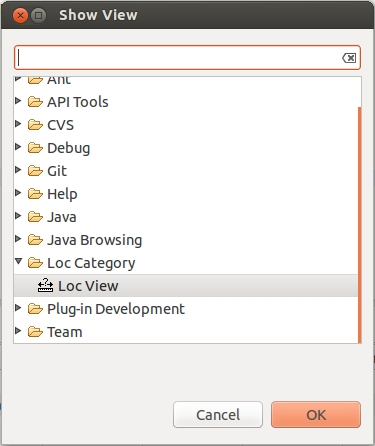
\includegraphics[width=0.5\textwidth]{graphics/wybor.jpg}
			\caption{Widok na wybór widoku wtyczki.}
			\label{fig:view_wybor}
		\end{figure}
				
		Po uruchomieniu wtyczki bêdzie dostêpny podstawowy widok historii plików w projektach. Na dole 
		okna uporz¹dkowane s¹ wszystkie projekty. Dla ka¿dej zak³adki wyœwietlone s¹ wszystkie pliki
		nale¿¹ce do danego projektu wraz histori¹ 5 ostatnich zmian w iloœci linii kodu (miara LOC).
		Je¿eli dla danego pliku nie istnieje zapis dla którejœ ze zmian wtedy zostaje wyœwietlony 
		znak \textit{x}. Widok pojedynczego projektu zosta³ pokazany na rysunku \ref{fig:view}. Mo¿na te¿
		zwin¹æ pliki nale¿¹ce do jednego z~projektów, wtedy bêdzie wyœwietlana tylko nazwa danego
		projektu.

		\begin{figure}[!htp]
			\centering
			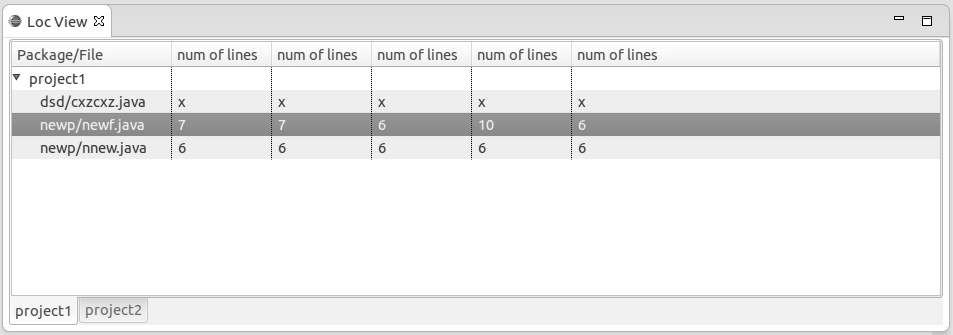
\includegraphics[width=0.8\textwidth]{graphics/view.jpg}
			\caption{Widok na podstawowy wygl¹d wtyczki.}
			\label{fig:view}
		\end{figure}

		Dostêp do pozosta³ej historii zmian plików dostêpny jest poprzez dwukrotne klikniêcie na nazwê
		pliku w widoku podstawowym. Operacja ta powoduje wyœwietlenie okna dialogowego z wykresami.
		Domyœlnie na pierwszym planie zostaje wyœwietlony wykres ostatnich 100 zmian danego pliku. Jeœli 
		plik posiada mniejsz¹ bazê zmian zostan¹ wyœwietlone wszystkie dostêpne dane. Widok zak³adki LOC
		przedstawiony jest na rysunku \ref{fig:LOC}.

		\begin{figure}[!htp]
			\centering
			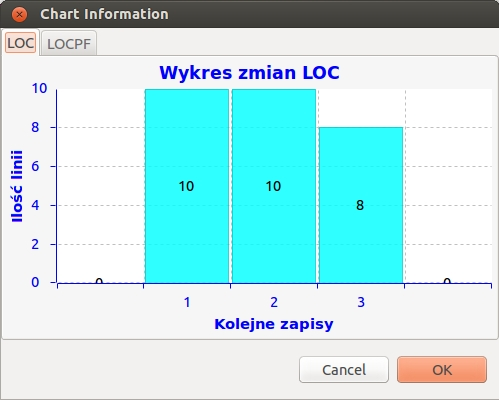
\includegraphics[width=0.5\textwidth]{graphics/chartLOC.jpg}
			\caption{Widok na okno wykresów LOC.}
			\label{fig:LOC}
		\end{figure}
		
		Na drugiej zak³adce zamieszczony jest wykres drugiej miary, mianowicie LOCPF. Iloœæ wyœwietlanych
		danych jest analogiczna do wykresu wskaŸnika LOC. Widok drugiego wykresu zosta³ zamieszczony na
		rysunku \ref{fig:LOCPF}.


		\begin{figure}[!htp]
			\centering
			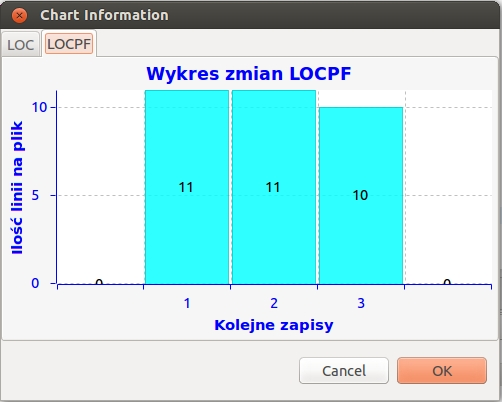
\includegraphics[width=0.5\textwidth]{graphics/chartLOCPF.jpg}
			\caption{Widok na okno wykresów LOCPF.}
			\label{fig:LOCPF}
		\end{figure}

\section{Podsumowanie}
\label{sec:podsumowanie}

Zaproponowane rozwi¹zanie pozwala œledziæ historiê dwóch wskaŸników: linii kodu w pliku i œredniej iloœci
linii kodu na plik w projekcie. Sposób wizualizacji pozwala w ³atwy sposób œledziæ rozwój projektu i obserwowaæ nie tylko ostatnie zmiany ale równie¿ du¿o wczeœniejsze etapy pracy.

Jako strukturê bazê danych wybrano plik xml. Takie podejœcie umo¿liwia prosty i czytelny zapis 
zmian. Dla bazy danych przyjêto model przyrostowy, tzn. ka¿da kolejna zmiana pliku zostaje 
dopisana nowym elementem w pliku xml. Wykorzystanie pliku xml, ³atwego do analizy, pozwala na 
wykorzystanie budowanej bazy nie tylko w tej wtyczce, ale mog¹ go wykorzystywaæ inne programy 
badaj¹ce prace programisty.

Niestety takie podejście nie jest pozbawione wad. Reprezentacja danych w formacie XML nie jest
optymalne pod względem zajętości pamięci. Poza tym konstrukcja programu zakłada, że plik jest
otwierany, parsowany i zamykany w każdej iteracji pracy programisty, gdzie iteracjami nazywa się
okresy między kolejnymi zapisaniami zmian w śledzonych plikach. Jest to również podejście 
nieoptymalne gdyż przy większych rozmiarach bazy danych, ciągłe parsowanie pliku xml, może być
bardzo obciążające dla procesora.

Ważną rzeczą, o której należy nie zapominać, jest łatwość użytkowania i płynność działania
oprogramowania służącego do pomiaru jakości pracy oraz kodu. Programista nie powinien odwracać 
swojej uwagi od głównego zadania jakim jest tworzenie kodu przez obecność programów takich jak
zaproponowana wtyczka. Pomiar pracy, agragacja danych i wstępna analizach powinna być 
transparentna dla programisty, a więc nie wymagać od niego dodatkowych cyklicznych akcji oraz
nie spowalniać pracy środowiska. Jednocześnie, dla osoby zainteresowanej wynikami, reprezenatcja
wyników powinna być czytelna i dobrze skategoryzowana.

Utworzona wtyczka rzuca światło na szerokie zagadnienie jakim jest pomiar jakości pracy 
programisty. Nietrudno jest wyobrazić sobie jakie możliwości analizy stwarzałoby obszerne 
narzędzie tego typu podłączone do środowiska programistycznego. Duże korporacje zajmujące się
wytwarzaniem oprogramowania, chętnie inwestują pieniądze w takie narzędzia w celu zwiększenia
wydajności pracy, oraz przede wszystkim jakości kodu.


\bibliography{bibliografia01} 
\addcontentsline{toc}{section}{Bibliografia}